% Created by tikzDevice version 0.10.1 on 2016-11-27 16:52:17
% !TEX encoding = UTF-8 Unicode
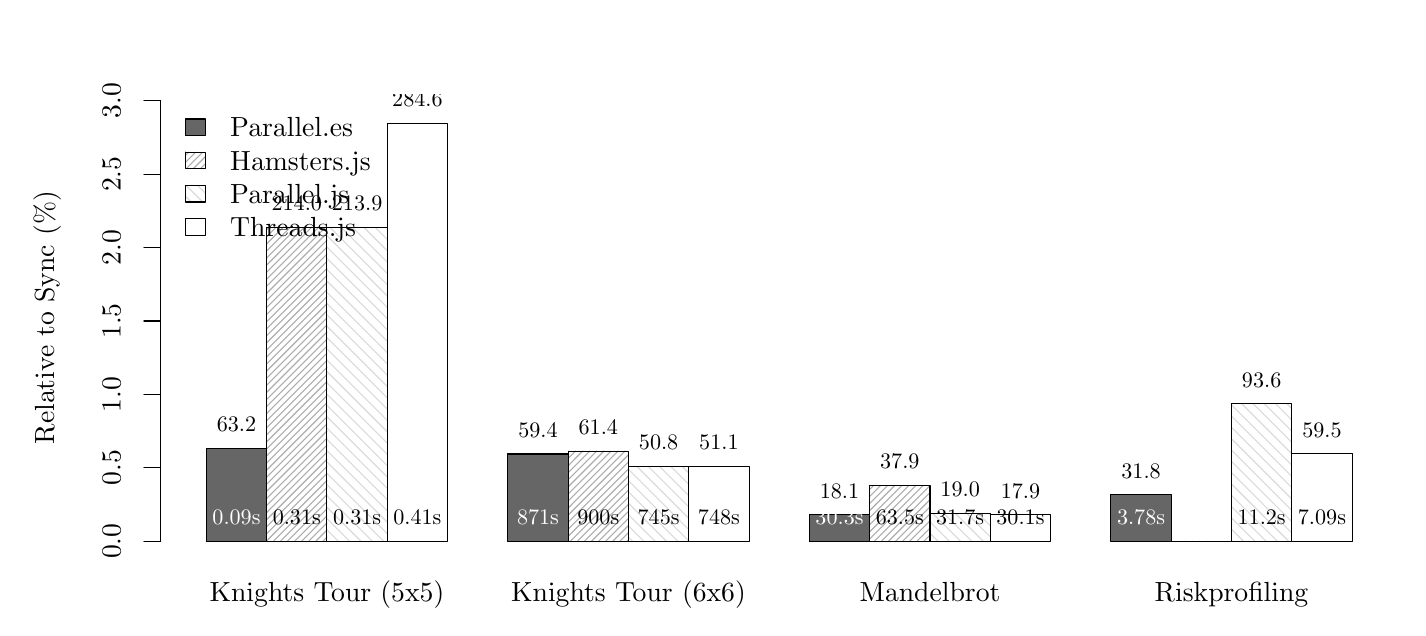
\begin{tikzpicture}[x=1pt,y=1pt]
\definecolor{fillColor}{RGB}{255,255,255}
\path[use as bounding box,fill=fillColor,fill opacity=0.00] (0,0) rectangle (495.15,209.58);
\begin{scope}
\path[clip] (  0.00,  0.00) rectangle (495.15,209.58);
\definecolor{fillColor}{gray}{0.40}

\path[fill=fillColor] ( 64.56, 24.00) --
	( 86.35, 24.00) --
	( 86.35, 57.51) --
	( 64.56, 57.51) --
	cycle;
\definecolor{drawColor}{RGB}{172,172,172}

\path[draw=drawColor,line width= 0.4pt,line join=round,line cap=round] ( 86.35,136.57) -- ( 87.30,137.52);

\path[draw=drawColor,line width= 0.4pt,line join=round,line cap=round] ( 86.35,134.01) -- ( 89.85,137.52);

\path[draw=drawColor,line width= 0.4pt,line join=round,line cap=round] ( 86.35,131.46) -- ( 92.41,137.52);

\path[draw=drawColor,line width= 0.4pt,line join=round,line cap=round] ( 86.35,128.90) -- ( 94.96,137.52);

\path[draw=drawColor,line width= 0.4pt,line join=round,line cap=round] ( 86.35,126.35) -- ( 97.52,137.52);

\path[draw=drawColor,line width= 0.4pt,line join=round,line cap=round] ( 86.35,123.79) -- (100.07,137.52);

\path[draw=drawColor,line width= 0.4pt,line join=round,line cap=round] ( 86.35,121.24) -- (102.63,137.52);

\path[draw=drawColor,line width= 0.4pt,line join=round,line cap=round] ( 86.35,118.68) -- (105.18,137.52);

\path[draw=drawColor,line width= 0.4pt,line join=round,line cap=round] ( 86.35,116.13) -- (107.74,137.52);

\path[draw=drawColor,line width= 0.4pt,line join=round,line cap=round] ( 86.35,113.57) -- (108.14,135.36);

\path[draw=drawColor,line width= 0.4pt,line join=round,line cap=round] ( 86.35,111.02) -- (108.14,132.81);

\path[draw=drawColor,line width= 0.4pt,line join=round,line cap=round] ( 86.35,108.46) -- (108.14,130.25);

\path[draw=drawColor,line width= 0.4pt,line join=round,line cap=round] ( 86.35,105.91) -- (108.14,127.70);

\path[draw=drawColor,line width= 0.4pt,line join=round,line cap=round] ( 86.35,103.35) -- (108.14,125.14);

\path[draw=drawColor,line width= 0.4pt,line join=round,line cap=round] ( 86.35,100.80) -- (108.14,122.59);

\path[draw=drawColor,line width= 0.4pt,line join=round,line cap=round] ( 86.35, 98.24) -- (108.14,120.03);

\path[draw=drawColor,line width= 0.4pt,line join=round,line cap=round] ( 86.35, 95.69) -- (108.14,117.48);

\path[draw=drawColor,line width= 0.4pt,line join=round,line cap=round] ( 86.35, 93.13) -- (108.14,114.92);

\path[draw=drawColor,line width= 0.4pt,line join=round,line cap=round] ( 86.35, 90.58) -- (108.14,112.37);

\path[draw=drawColor,line width= 0.4pt,line join=round,line cap=round] ( 86.35, 88.02) -- (108.14,109.81);

\path[draw=drawColor,line width= 0.4pt,line join=round,line cap=round] ( 86.35, 85.47) -- (108.14,107.26);

\path[draw=drawColor,line width= 0.4pt,line join=round,line cap=round] ( 86.35, 82.91) -- (108.14,104.70);

\path[draw=drawColor,line width= 0.4pt,line join=round,line cap=round] ( 86.35, 80.36) -- (108.14,102.15);

\path[draw=drawColor,line width= 0.4pt,line join=round,line cap=round] ( 86.35, 77.80) -- (108.14, 99.59);

\path[draw=drawColor,line width= 0.4pt,line join=round,line cap=round] ( 86.35, 75.25) -- (108.14, 97.04);

\path[draw=drawColor,line width= 0.4pt,line join=round,line cap=round] ( 86.35, 72.69) -- (108.14, 94.48);

\path[draw=drawColor,line width= 0.4pt,line join=round,line cap=round] ( 86.35, 70.14) -- (108.14, 91.93);

\path[draw=drawColor,line width= 0.4pt,line join=round,line cap=round] ( 86.35, 67.58) -- (108.14, 89.37);

\path[draw=drawColor,line width= 0.4pt,line join=round,line cap=round] ( 86.35, 65.03) -- (108.14, 86.82);

\path[draw=drawColor,line width= 0.4pt,line join=round,line cap=round] ( 86.35, 62.47) -- (108.14, 84.26);

\path[draw=drawColor,line width= 0.4pt,line join=round,line cap=round] ( 86.35, 59.92) -- (108.14, 81.71);

\path[draw=drawColor,line width= 0.4pt,line join=round,line cap=round] ( 86.35, 57.36) -- (108.14, 79.15);

\path[draw=drawColor,line width= 0.4pt,line join=round,line cap=round] ( 86.35, 54.81) -- (108.14, 76.60);

\path[draw=drawColor,line width= 0.4pt,line join=round,line cap=round] ( 86.35, 52.25) -- (108.14, 74.04);

\path[draw=drawColor,line width= 0.4pt,line join=round,line cap=round] ( 86.35, 49.70) -- (108.14, 71.49);

\path[draw=drawColor,line width= 0.4pt,line join=round,line cap=round] ( 86.35, 47.14) -- (108.14, 68.93);

\path[draw=drawColor,line width= 0.4pt,line join=round,line cap=round] ( 86.35, 44.59) -- (108.14, 66.38);

\path[draw=drawColor,line width= 0.4pt,line join=round,line cap=round] ( 86.35, 42.03) -- (108.14, 63.82);

\path[draw=drawColor,line width= 0.4pt,line join=round,line cap=round] ( 86.35, 39.48) -- (108.14, 61.27);

\path[draw=drawColor,line width= 0.4pt,line join=round,line cap=round] ( 86.35, 36.92) -- (108.14, 58.71);

\path[draw=drawColor,line width= 0.4pt,line join=round,line cap=round] ( 86.35, 34.36) -- (108.14, 56.16);

\path[draw=drawColor,line width= 0.4pt,line join=round,line cap=round] ( 86.35, 31.81) -- (108.14, 53.60);

\path[draw=drawColor,line width= 0.4pt,line join=round,line cap=round] ( 86.35, 29.25) -- (108.14, 51.05);

\path[draw=drawColor,line width= 0.4pt,line join=round,line cap=round] ( 86.35, 26.70) -- (108.14, 48.49);

\path[draw=drawColor,line width= 0.4pt,line join=round,line cap=round] ( 86.35, 24.14) -- (108.14, 45.94);

\path[draw=drawColor,line width= 0.4pt,line join=round,line cap=round] ( 88.76, 24.00) -- (108.14, 43.38);

\path[draw=drawColor,line width= 0.4pt,line join=round,line cap=round] ( 91.32, 24.00) -- (108.14, 40.82);

\path[draw=drawColor,line width= 0.4pt,line join=round,line cap=round] ( 93.87, 24.00) -- (108.14, 38.27);

\path[draw=drawColor,line width= 0.4pt,line join=round,line cap=round] ( 96.43, 24.00) -- (108.14, 35.71);

\path[draw=drawColor,line width= 0.4pt,line join=round,line cap=round] ( 98.98, 24.00) -- (108.14, 33.16);

\path[draw=drawColor,line width= 0.4pt,line join=round,line cap=round] (101.54, 24.00) -- (108.14, 30.60);

\path[draw=drawColor,line width= 0.4pt,line join=round,line cap=round] (104.09, 24.00) -- (108.14, 28.05);

\path[draw=drawColor,line width= 0.4pt,line join=round,line cap=round] (106.65, 24.00) -- (108.14, 25.49);
\definecolor{drawColor}{RGB}{218,218,218}

\path[draw=drawColor,line width= 0.4pt,line join=round,line cap=round] (108.18, 24.00) -- (108.14, 24.04);

\path[draw=drawColor,line width= 0.4pt,line join=round,line cap=round] (112.27, 24.00) -- (108.14, 28.13);

\path[draw=drawColor,line width= 0.4pt,line join=round,line cap=round] (116.36, 24.00) -- (108.14, 32.22);

\path[draw=drawColor,line width= 0.4pt,line join=round,line cap=round] (120.45, 24.00) -- (108.14, 36.30);

\path[draw=drawColor,line width= 0.4pt,line join=round,line cap=round] (124.53, 24.00) -- (108.14, 40.39);

\path[draw=drawColor,line width= 0.4pt,line join=round,line cap=round] (128.62, 24.00) -- (108.14, 44.48);

\path[draw=drawColor,line width= 0.4pt,line join=round,line cap=round] (129.93, 26.78) -- (108.14, 48.57);

\path[draw=drawColor,line width= 0.4pt,line join=round,line cap=round] (129.93, 30.87) -- (108.14, 52.66);

\path[draw=drawColor,line width= 0.4pt,line join=round,line cap=round] (129.93, 34.95) -- (108.14, 56.74);

\path[draw=drawColor,line width= 0.4pt,line join=round,line cap=round] (129.93, 39.04) -- (108.14, 60.83);

\path[draw=drawColor,line width= 0.4pt,line join=round,line cap=round] (129.93, 43.13) -- (108.14, 64.92);

\path[draw=drawColor,line width= 0.4pt,line join=round,line cap=round] (129.93, 47.22) -- (108.14, 69.01);

\path[draw=drawColor,line width= 0.4pt,line join=round,line cap=round] (129.93, 51.31) -- (108.14, 73.10);

\path[draw=drawColor,line width= 0.4pt,line join=round,line cap=round] (129.93, 55.39) -- (108.14, 77.19);

\path[draw=drawColor,line width= 0.4pt,line join=round,line cap=round] (129.93, 59.48) -- (108.14, 81.27);

\path[draw=drawColor,line width= 0.4pt,line join=round,line cap=round] (129.93, 63.57) -- (108.14, 85.36);

\path[draw=drawColor,line width= 0.4pt,line join=round,line cap=round] (129.93, 67.66) -- (108.14, 89.45);

\path[draw=drawColor,line width= 0.4pt,line join=round,line cap=round] (129.93, 71.75) -- (108.14, 93.54);

\path[draw=drawColor,line width= 0.4pt,line join=round,line cap=round] (129.93, 75.84) -- (108.14, 97.63);

\path[draw=drawColor,line width= 0.4pt,line join=round,line cap=round] (129.93, 79.92) -- (108.14,101.71);

\path[draw=drawColor,line width= 0.4pt,line join=round,line cap=round] (129.93, 84.01) -- (108.14,105.80);

\path[draw=drawColor,line width= 0.4pt,line join=round,line cap=round] (129.93, 88.10) -- (108.14,109.89);

\path[draw=drawColor,line width= 0.4pt,line join=round,line cap=round] (129.93, 92.19) -- (108.14,113.98);

\path[draw=drawColor,line width= 0.4pt,line join=round,line cap=round] (129.93, 96.28) -- (108.14,118.07);

\path[draw=drawColor,line width= 0.4pt,line join=round,line cap=round] (129.93,100.37) -- (108.14,122.16);

\path[draw=drawColor,line width= 0.4pt,line join=round,line cap=round] (129.93,104.45) -- (108.14,126.24);

\path[draw=drawColor,line width= 0.4pt,line join=round,line cap=round] (129.93,108.54) -- (108.14,130.33);

\path[draw=drawColor,line width= 0.4pt,line join=round,line cap=round] (129.93,112.63) -- (108.14,134.42);

\path[draw=drawColor,line width= 0.4pt,line join=round,line cap=round] (129.93,116.72) -- (109.19,137.46);

\path[draw=drawColor,line width= 0.4pt,line join=round,line cap=round] (129.93,120.81) -- (113.28,137.46);

\path[draw=drawColor,line width= 0.4pt,line join=round,line cap=round] (129.93,124.89) -- (117.36,137.46);

\path[draw=drawColor,line width= 0.4pt,line join=round,line cap=round] (129.93,128.98) -- (121.45,137.46);

\path[draw=drawColor,line width= 0.4pt,line join=round,line cap=round] (129.93,133.07) -- (125.54,137.46);

\path[draw=drawColor,line width= 0.4pt,line join=round,line cap=round] (129.93,137.16) -- (129.63,137.46);

\path[fill=fillColor] (173.51, 24.00) --
	(195.31, 24.00) --
	(195.31, 55.54) --
	(173.51, 55.54) --
	cycle;
\definecolor{drawColor}{RGB}{172,172,172}

\path[draw=drawColor,line width= 0.4pt,line join=round,line cap=round] (195.31, 56.44) -- (195.44, 56.58);

\path[draw=drawColor,line width= 0.4pt,line join=round,line cap=round] (195.31, 53.89) -- (198.00, 56.58);

\path[draw=drawColor,line width= 0.4pt,line join=round,line cap=round] (195.31, 51.33) -- (200.55, 56.58);

\path[draw=drawColor,line width= 0.4pt,line join=round,line cap=round] (195.31, 48.78) -- (203.11, 56.58);

\path[draw=drawColor,line width= 0.4pt,line join=round,line cap=round] (195.31, 46.22) -- (205.66, 56.58);

\path[draw=drawColor,line width= 0.4pt,line join=round,line cap=round] (195.31, 43.67) -- (208.22, 56.58);

\path[draw=drawColor,line width= 0.4pt,line join=round,line cap=round] (195.31, 41.11) -- (210.77, 56.58);

\path[draw=drawColor,line width= 0.4pt,line join=round,line cap=round] (195.31, 38.56) -- (213.33, 56.58);

\path[draw=drawColor,line width= 0.4pt,line join=round,line cap=round] (195.31, 36.00) -- (215.88, 56.58);

\path[draw=drawColor,line width= 0.4pt,line join=round,line cap=round] (195.31, 33.45) -- (217.10, 55.24);

\path[draw=drawColor,line width= 0.4pt,line join=round,line cap=round] (195.31, 30.89) -- (217.10, 52.68);

\path[draw=drawColor,line width= 0.4pt,line join=round,line cap=round] (195.31, 28.34) -- (217.10, 50.13);

\path[draw=drawColor,line width= 0.4pt,line join=round,line cap=round] (195.31, 25.78) -- (217.10, 47.57);

\path[draw=drawColor,line width= 0.4pt,line join=round,line cap=round] (196.08, 24.00) -- (217.10, 45.02);

\path[draw=drawColor,line width= 0.4pt,line join=round,line cap=round] (198.63, 24.00) -- (217.10, 42.46);

\path[draw=drawColor,line width= 0.4pt,line join=round,line cap=round] (201.19, 24.00) -- (217.10, 39.91);

\path[draw=drawColor,line width= 0.4pt,line join=round,line cap=round] (203.74, 24.00) -- (217.10, 37.35);

\path[draw=drawColor,line width= 0.4pt,line join=round,line cap=round] (206.30, 24.00) -- (217.10, 34.80);

\path[draw=drawColor,line width= 0.4pt,line join=round,line cap=round] (208.85, 24.00) -- (217.10, 32.24);

\path[draw=drawColor,line width= 0.4pt,line join=round,line cap=round] (211.41, 24.00) -- (217.10, 29.69);

\path[draw=drawColor,line width= 0.4pt,line join=round,line cap=round] (213.96, 24.00) -- (217.10, 27.13);

\path[draw=drawColor,line width= 0.4pt,line join=round,line cap=round] (216.52, 24.00) -- (217.10, 24.58);
\definecolor{drawColor}{RGB}{218,218,218}

\path[draw=drawColor,line width= 0.4pt,line join=round,line cap=round] (218.56, 24.00) -- (217.10, 25.47);

\path[draw=drawColor,line width= 0.4pt,line join=round,line cap=round] (222.65, 24.00) -- (217.10, 29.55);

\path[draw=drawColor,line width= 0.4pt,line join=round,line cap=round] (226.74, 24.00) -- (217.10, 33.64);

\path[draw=drawColor,line width= 0.4pt,line join=round,line cap=round] (230.83, 24.00) -- (217.10, 37.73);

\path[draw=drawColor,line width= 0.4pt,line join=round,line cap=round] (234.92, 24.00) -- (217.10, 41.82);

\path[draw=drawColor,line width= 0.4pt,line join=round,line cap=round] (238.89, 24.12) -- (217.10, 45.91);

\path[draw=drawColor,line width= 0.4pt,line join=round,line cap=round] (238.89, 28.21) -- (217.10, 50.00);

\path[draw=drawColor,line width= 0.4pt,line join=round,line cap=round] (238.89, 32.29) -- (220.20, 50.98);

\path[draw=drawColor,line width= 0.4pt,line join=round,line cap=round] (238.89, 36.38) -- (224.29, 50.98);

\path[draw=drawColor,line width= 0.4pt,line join=round,line cap=round] (238.89, 40.47) -- (228.38, 50.98);

\path[draw=drawColor,line width= 0.4pt,line join=round,line cap=round] (238.89, 44.56) -- (232.47, 50.98);

\path[draw=drawColor,line width= 0.4pt,line join=round,line cap=round] (238.89, 48.65) -- (236.55, 50.98);

\path[fill=fillColor] (282.47, 24.00) --
	(304.26, 24.00) --
	(304.26, 33.59) --
	(282.47, 33.59) --
	cycle;
\definecolor{drawColor}{RGB}{172,172,172}

\path[draw=drawColor,line width= 0.4pt,line join=round,line cap=round] (304.26, 42.75) -- (305.62, 44.12);

\path[draw=drawColor,line width= 0.4pt,line join=round,line cap=round] (304.26, 40.20) -- (308.18, 44.12);

\path[draw=drawColor,line width= 0.4pt,line join=round,line cap=round] (304.26, 37.64) -- (310.73, 44.12);

\path[draw=drawColor,line width= 0.4pt,line join=round,line cap=round] (304.26, 35.09) -- (313.29, 44.12);

\path[draw=drawColor,line width= 0.4pt,line join=round,line cap=round] (304.26, 32.53) -- (315.84, 44.12);

\path[draw=drawColor,line width= 0.4pt,line join=round,line cap=round] (304.26, 29.98) -- (318.40, 44.12);

\path[draw=drawColor,line width= 0.4pt,line join=round,line cap=round] (304.26, 27.42) -- (320.95, 44.12);

\path[draw=drawColor,line width= 0.4pt,line join=round,line cap=round] (304.26, 24.87) -- (323.51, 44.12);

\path[draw=drawColor,line width= 0.4pt,line join=round,line cap=round] (305.95, 24.00) -- (326.05, 44.10);

\path[draw=drawColor,line width= 0.4pt,line join=round,line cap=round] (308.50, 24.00) -- (326.05, 41.55);

\path[draw=drawColor,line width= 0.4pt,line join=round,line cap=round] (311.06, 24.00) -- (326.05, 38.99);

\path[draw=drawColor,line width= 0.4pt,line join=round,line cap=round] (313.61, 24.00) -- (326.05, 36.44);

\path[draw=drawColor,line width= 0.4pt,line join=round,line cap=round] (316.17, 24.00) -- (326.05, 33.88);

\path[draw=drawColor,line width= 0.4pt,line join=round,line cap=round] (318.72, 24.00) -- (326.05, 31.33);

\path[draw=drawColor,line width= 0.4pt,line join=round,line cap=round] (321.28, 24.00) -- (326.05, 28.77);

\path[draw=drawColor,line width= 0.4pt,line join=round,line cap=round] (323.83, 24.00) -- (326.05, 26.22);
\definecolor{drawColor}{RGB}{218,218,218}

\path[draw=drawColor,line width= 0.4pt,line join=round,line cap=round] (328.94, 24.00) -- (326.05, 26.89);

\path[draw=drawColor,line width= 0.4pt,line join=round,line cap=round] (333.03, 24.00) -- (326.05, 30.98);

\path[draw=drawColor,line width= 0.4pt,line join=round,line cap=round] (337.12, 24.00) -- (327.07, 34.06);

\path[draw=drawColor,line width= 0.4pt,line join=round,line cap=round] (341.21, 24.00) -- (331.15, 34.06);

\path[draw=drawColor,line width= 0.4pt,line join=round,line cap=round] (345.30, 24.00) -- (335.24, 34.06);

\path[draw=drawColor,line width= 0.4pt,line join=round,line cap=round] (347.84, 25.54) -- (339.33, 34.06);

\path[draw=drawColor,line width= 0.4pt,line join=round,line cap=round] (347.84, 29.63) -- (343.42, 34.06);

\path[draw=drawColor,line width= 0.4pt,line join=round,line cap=round] (347.84, 33.72) -- (347.51, 34.06);

\path[fill=fillColor] (391.42, 24.00) --
	(413.21, 24.00) --
	(413.21, 40.85) --
	(391.42, 40.85) --
	cycle;
\definecolor{drawColor}{RGB}{172,172,172}

\path[draw=drawColor,line width= 0.4pt,line join=round,line cap=round] (413.26, 24.00) -- (413.26, 24.00);

\path[draw=drawColor,line width= 0.4pt,line join=round,line cap=round] (415.82, 24.00) -- (415.82, 24.00);

\path[draw=drawColor,line width= 0.4pt,line join=round,line cap=round] (418.37, 24.00) -- (418.37, 24.00);

\path[draw=drawColor,line width= 0.4pt,line join=round,line cap=round] (420.93, 24.00) -- (420.93, 24.00);

\path[draw=drawColor,line width= 0.4pt,line join=round,line cap=round] (423.48, 24.00) -- (423.48, 24.00);

\path[draw=drawColor,line width= 0.4pt,line join=round,line cap=round] (426.04, 24.00) -- (426.04, 24.00);

\path[draw=drawColor,line width= 0.4pt,line join=round,line cap=round] (428.59, 24.00) -- (428.59, 24.00);

\path[draw=drawColor,line width= 0.4pt,line join=round,line cap=round] (431.15, 24.00) -- (431.15, 24.00);

\path[draw=drawColor,line width= 0.4pt,line join=round,line cap=round] (433.71, 24.00) -- (433.71, 24.00);
\definecolor{drawColor}{RGB}{218,218,218}

\path[draw=drawColor,line width= 0.4pt,line join=round,line cap=round] (435.24, 24.00) -- (435.00, 24.23);

\path[draw=drawColor,line width= 0.4pt,line join=round,line cap=round] (439.33, 24.00) -- (435.00, 28.32);

\path[draw=drawColor,line width= 0.4pt,line join=round,line cap=round] (443.41, 24.00) -- (435.00, 32.41);

\path[draw=drawColor,line width= 0.4pt,line join=round,line cap=round] (447.50, 24.00) -- (435.00, 36.50);

\path[draw=drawColor,line width= 0.4pt,line join=round,line cap=round] (451.59, 24.00) -- (435.00, 40.59);

\path[draw=drawColor,line width= 0.4pt,line join=round,line cap=round] (455.68, 24.00) -- (435.00, 44.67);

\path[draw=drawColor,line width= 0.4pt,line join=round,line cap=round] (456.80, 26.97) -- (435.00, 48.76);

\path[draw=drawColor,line width= 0.4pt,line join=round,line cap=round] (456.80, 31.06) -- (435.00, 52.85);

\path[draw=drawColor,line width= 0.4pt,line join=round,line cap=round] (456.80, 35.15) -- (435.00, 56.94);

\path[draw=drawColor,line width= 0.4pt,line join=round,line cap=round] (456.80, 39.24) -- (435.00, 61.03);

\path[draw=drawColor,line width= 0.4pt,line join=round,line cap=round] (456.80, 43.33) -- (435.00, 65.12);

\path[draw=drawColor,line width= 0.4pt,line join=round,line cap=round] (456.80, 47.41) -- (435.00, 69.20);

\path[draw=drawColor,line width= 0.4pt,line join=round,line cap=round] (456.80, 51.50) -- (435.00, 73.29);

\path[draw=drawColor,line width= 0.4pt,line join=round,line cap=round] (456.80, 55.59) -- (438.71, 73.68);

\path[draw=drawColor,line width= 0.4pt,line join=round,line cap=round] (456.80, 59.68) -- (442.79, 73.68);

\path[draw=drawColor,line width= 0.4pt,line join=round,line cap=round] (456.80, 63.77) -- (446.88, 73.68);

\path[draw=drawColor,line width= 0.4pt,line join=round,line cap=round] (456.80, 67.85) -- (450.97, 73.68);

\path[draw=drawColor,line width= 0.4pt,line join=round,line cap=round] (456.80, 71.94) -- (455.06, 73.68);
\definecolor{drawColor}{RGB}{0,0,0}

\path[draw=drawColor,line width= 0.4pt,line join=round,line cap=round] ( 64.56, 24.00) --
	( 86.35, 24.00) --
	( 86.35, 57.51) --
	( 64.56, 57.51) --
	( 64.56, 24.00);

\path[draw=drawColor,line width= 0.4pt,line join=round,line cap=round] ( 86.35, 24.00) --
	(108.14, 24.00) --
	(108.14,137.52) --
	( 86.35,137.52) --
	( 86.35, 24.00);

\path[draw=drawColor,line width= 0.4pt,line join=round,line cap=round] (108.14, 24.00) --
	(129.93, 24.00) --
	(129.93,137.46) --
	(108.14,137.46) --
	(108.14, 24.00);

\path[draw=drawColor,line width= 0.4pt,line join=round,line cap=round] (129.93, 24.00) --
	(151.72, 24.00) --
	(151.72,174.97) --
	(129.93,174.97) --
	(129.93, 24.00);

\path[draw=drawColor,line width= 0.4pt,line join=round,line cap=round] (173.51, 24.00) --
	(195.31, 24.00) --
	(195.31, 55.54) --
	(173.51, 55.54) --
	(173.51, 24.00);

\path[draw=drawColor,line width= 0.4pt,line join=round,line cap=round] (195.31, 24.00) --
	(217.10, 24.00) --
	(217.10, 56.58) --
	(195.31, 56.58) --
	(195.31, 24.00);

\path[draw=drawColor,line width= 0.4pt,line join=round,line cap=round] (217.10, 24.00) --
	(238.89, 24.00) --
	(238.89, 50.98) --
	(217.10, 50.98) --
	(217.10, 24.00);

\path[draw=drawColor,line width= 0.4pt,line join=round,line cap=round] (238.89, 24.00) --
	(260.68, 24.00) --
	(260.68, 51.09) --
	(238.89, 51.09) --
	(238.89, 24.00);

\path[draw=drawColor,line width= 0.4pt,line join=round,line cap=round] (282.47, 24.00) --
	(304.26, 24.00) --
	(304.26, 33.59) --
	(282.47, 33.59) --
	(282.47, 24.00);

\path[draw=drawColor,line width= 0.4pt,line join=round,line cap=round] (304.26, 24.00) --
	(326.05, 24.00) --
	(326.05, 44.12) --
	(304.26, 44.12) --
	(304.26, 24.00);

\path[draw=drawColor,line width= 0.4pt,line join=round,line cap=round] (326.05, 24.00) --
	(347.84, 24.00) --
	(347.84, 34.06) --
	(326.05, 34.06) --
	(326.05, 24.00);

\path[draw=drawColor,line width= 0.4pt,line join=round,line cap=round] (347.84, 24.00) --
	(369.63, 24.00) --
	(369.63, 33.52) --
	(347.84, 33.52) --
	(347.84, 24.00);

\path[draw=drawColor,line width= 0.4pt,line join=round,line cap=round] (391.42, 24.00) --
	(413.21, 24.00) --
	(413.21, 40.85) --
	(391.42, 40.85) --
	(391.42, 24.00);

\path[draw=drawColor,line width= 0.4pt,line join=round,line cap=round] (413.21, 24.00) --
	(435.00, 24.00) --
	(413.21, 24.00);

\path[draw=drawColor,line width= 0.4pt,line join=round,line cap=round] (435.00, 24.00) --
	(456.80, 24.00) --
	(456.80, 73.68) --
	(435.00, 73.68) --
	(435.00, 24.00);

\path[draw=drawColor,line width= 0.4pt,line join=round,line cap=round] (456.80, 24.00) --
	(478.59, 24.00) --
	(478.59, 55.57) --
	(456.80, 55.57) --
	(456.80, 24.00);
\end{scope}
\begin{scope}
\path[clip] (  0.00,  0.00) rectangle (495.15,209.58);
\definecolor{drawColor}{RGB}{0,0,0}

\node[text=drawColor,anchor=base,inner sep=0pt, outer sep=0pt, scale=  1.00] at (108.14,  2.40) {Knights Tour (5x5)};

\node[text=drawColor,anchor=base,inner sep=0pt, outer sep=0pt, scale=  1.00] at (217.10,  2.40) {Knights Tour (6x6)};

\node[text=drawColor,anchor=base,inner sep=0pt, outer sep=0pt, scale=  1.00] at (326.05,  2.40) {Mandelbrot};

\node[text=drawColor,anchor=base,inner sep=0pt, outer sep=0pt, scale=  1.00] at (435.00,  2.40) {Riskprofiling};
\end{scope}
\begin{scope}
\path[clip] (  0.00,  0.00) rectangle (495.15,209.58);
\definecolor{drawColor}{RGB}{0,0,0}

\node[text=drawColor,rotate= 90.00,anchor=base,inner sep=0pt, outer sep=0pt, scale=  1.00] at (  9.60,104.79) {Relative to Sync ({\%})};
\end{scope}
\begin{scope}
\path[clip] (  0.00,  0.00) rectangle (495.15,209.58);
\definecolor{drawColor}{RGB}{0,0,0}

\path[draw=drawColor,line width= 0.4pt,line join=round,line cap=round] ( 48.00, 24.00) -- ( 48.00,183.17);

\path[draw=drawColor,line width= 0.4pt,line join=round,line cap=round] ( 48.00, 24.00) -- ( 42.00, 24.00);

\path[draw=drawColor,line width= 0.4pt,line join=round,line cap=round] ( 48.00, 50.53) -- ( 42.00, 50.53);

\path[draw=drawColor,line width= 0.4pt,line join=round,line cap=round] ( 48.00, 77.06) -- ( 42.00, 77.06);

\path[draw=drawColor,line width= 0.4pt,line join=round,line cap=round] ( 48.00,103.58) -- ( 42.00,103.58);

\path[draw=drawColor,line width= 0.4pt,line join=round,line cap=round] ( 48.00,130.11) -- ( 42.00,130.11);

\path[draw=drawColor,line width= 0.4pt,line join=round,line cap=round] ( 48.00,156.64) -- ( 42.00,156.64);

\path[draw=drawColor,line width= 0.4pt,line join=round,line cap=round] ( 48.00,183.17) -- ( 42.00,183.17);

\node[text=drawColor,rotate= 90.00,anchor=base,inner sep=0pt, outer sep=0pt, scale=  1.00] at ( 33.60, 24.00) {0.0};

\node[text=drawColor,rotate= 90.00,anchor=base,inner sep=0pt, outer sep=0pt, scale=  1.00] at ( 33.60, 50.53) {0.5};

\node[text=drawColor,rotate= 90.00,anchor=base,inner sep=0pt, outer sep=0pt, scale=  1.00] at ( 33.60, 77.06) {1.0};

\node[text=drawColor,rotate= 90.00,anchor=base,inner sep=0pt, outer sep=0pt, scale=  1.00] at ( 33.60,103.58) {1.5};

\node[text=drawColor,rotate= 90.00,anchor=base,inner sep=0pt, outer sep=0pt, scale=  1.00] at ( 33.60,130.11) {2.0};

\node[text=drawColor,rotate= 90.00,anchor=base,inner sep=0pt, outer sep=0pt, scale=  1.00] at ( 33.60,156.64) {2.5};

\node[text=drawColor,rotate= 90.00,anchor=base,inner sep=0pt, outer sep=0pt, scale=  1.00] at ( 33.60,183.17) {3.0};
\end{scope}
\begin{scope}
\path[clip] ( 48.00, 24.00) rectangle (495.15,185.58);
\definecolor{fillColor}{gray}{0.40}

\path[fill=fillColor] ( 57.00,176.58) --
	( 64.20,176.58) --
	( 64.20,170.58) --
	( 57.00,170.58) --
	cycle;
\definecolor{drawColor}{RGB}{172,172,172}

\path[draw=drawColor,line width= 0.4pt,line join=round,line cap=round] ( 57.00,163.43) -- ( 58.15,164.58);

\path[draw=drawColor,line width= 0.4pt,line join=round,line cap=round] ( 57.00,160.88) -- ( 60.71,164.58);

\path[draw=drawColor,line width= 0.4pt,line join=round,line cap=round] ( 57.26,158.58) -- ( 63.26,164.58);

\path[draw=drawColor,line width= 0.4pt,line join=round,line cap=round] ( 59.82,158.58) -- ( 64.20,162.97);

\path[draw=drawColor,line width= 0.4pt,line join=round,line cap=round] ( 62.37,158.58) -- ( 64.20,160.41);
\definecolor{drawColor}{RGB}{218,218,218}

\path[draw=drawColor,line width= 0.4pt,line join=round,line cap=round] ( 59.19,146.58) -- ( 57.00,148.77);

\path[draw=drawColor,line width= 0.4pt,line join=round,line cap=round] ( 63.27,146.58) -- ( 57.27,152.58);

\path[draw=drawColor,line width= 0.4pt,line join=round,line cap=round] ( 64.20,149.75) -- ( 61.36,152.58);
\definecolor{drawColor}{RGB}{0,0,0}

\path[draw=drawColor,line width= 0.4pt,line join=round,line cap=round] ( 57.00,176.58) --
	( 64.20,176.58) --
	( 64.20,170.58) --
	( 57.00,170.58) --
	( 57.00,176.58);

\path[draw=drawColor,line width= 0.4pt,line join=round,line cap=round] ( 57.00,164.58) --
	( 64.20,164.58) --
	( 64.20,158.58) --
	( 57.00,158.58) --
	( 57.00,164.58);

\path[draw=drawColor,line width= 0.4pt,line join=round,line cap=round] ( 57.00,152.58) --
	( 64.20,152.58) --
	( 64.20,146.58) --
	( 57.00,146.58) --
	( 57.00,152.58);

\path[draw=drawColor,line width= 0.4pt,line join=round,line cap=round] ( 57.00,140.58) --
	( 64.20,140.58) --
	( 64.20,134.58) --
	( 57.00,134.58) --
	( 57.00,140.58);

\node[text=drawColor,anchor=base west,inner sep=0pt, outer sep=0pt, scale=  1.00] at ( 73.20,170.14) {Parallel.es};

\node[text=drawColor,anchor=base west,inner sep=0pt, outer sep=0pt, scale=  1.00] at ( 73.20,158.14) {Hamsters.js};

\node[text=drawColor,anchor=base west,inner sep=0pt, outer sep=0pt, scale=  1.00] at ( 73.20,146.14) {Parallel.js};

\node[text=drawColor,anchor=base west,inner sep=0pt, outer sep=0pt, scale=  1.00] at ( 73.20,134.14) {Threads.js};

\node[text=drawColor,anchor=base,inner sep=0pt, outer sep=0pt, scale=  0.80] at ( 75.46, 63.51) {63.2};

\node[text=drawColor,anchor=base,inner sep=0pt, outer sep=0pt, scale=  0.80] at ( 97.25,143.52) {214.0};

\node[text=drawColor,anchor=base,inner sep=0pt, outer sep=0pt, scale=  0.80] at (119.04,143.46) {213.9};

\node[text=drawColor,anchor=base,inner sep=0pt, outer sep=0pt, scale=  0.80] at (140.83,180.97) {284.6};

\node[text=drawColor,anchor=base,inner sep=0pt, outer sep=0pt, scale=  0.80] at (184.41, 61.54) {59.4};

\node[text=drawColor,anchor=base,inner sep=0pt, outer sep=0pt, scale=  0.80] at (206.20, 62.58) {61.4};

\node[text=drawColor,anchor=base,inner sep=0pt, outer sep=0pt, scale=  0.80] at (227.99, 56.98) {50.8};

\node[text=drawColor,anchor=base,inner sep=0pt, outer sep=0pt, scale=  0.80] at (249.78, 57.09) {51.1};

\node[text=drawColor,anchor=base,inner sep=0pt, outer sep=0pt, scale=  0.80] at (293.36, 39.59) {18.1};

\node[text=drawColor,anchor=base,inner sep=0pt, outer sep=0pt, scale=  0.80] at (315.16, 50.12) {37.9};

\node[text=drawColor,anchor=base,inner sep=0pt, outer sep=0pt, scale=  0.80] at (336.95, 40.06) {19.0};

\node[text=drawColor,anchor=base,inner sep=0pt, outer sep=0pt, scale=  0.80] at (358.74, 39.52) {17.9};

\node[text=drawColor,anchor=base,inner sep=0pt, outer sep=0pt, scale=  0.80] at (402.32, 46.85) {31.8};

\node[text=drawColor,anchor=base,inner sep=0pt, outer sep=0pt, scale=  0.80] at (445.90, 79.68) {93.6};

\node[text=drawColor,anchor=base,inner sep=0pt, outer sep=0pt, scale=  0.80] at (467.69, 61.57) {59.5};
\definecolor{drawColor}{RGB}{255,255,255}

\node[text=drawColor,anchor=base,inner sep=0pt, outer sep=0pt, scale=  0.80] at ( 75.46, 30.00) {0.09s};
\definecolor{drawColor}{RGB}{0,0,0}

\node[text=drawColor,anchor=base,inner sep=0pt, outer sep=0pt, scale=  0.80] at ( 97.25, 30.00) {0.31s};

\node[text=drawColor,anchor=base,inner sep=0pt, outer sep=0pt, scale=  0.80] at (119.04, 30.00) {0.31s};

\node[text=drawColor,anchor=base,inner sep=0pt, outer sep=0pt, scale=  0.80] at (140.83, 30.00) {0.41s};
\definecolor{drawColor}{RGB}{255,255,255}

\node[text=drawColor,anchor=base,inner sep=0pt, outer sep=0pt, scale=  0.80] at (184.41, 30.00) {871s};
\definecolor{drawColor}{RGB}{0,0,0}

\node[text=drawColor,anchor=base,inner sep=0pt, outer sep=0pt, scale=  0.80] at (206.20, 30.00) {900s};

\node[text=drawColor,anchor=base,inner sep=0pt, outer sep=0pt, scale=  0.80] at (227.99, 30.00) {745s};

\node[text=drawColor,anchor=base,inner sep=0pt, outer sep=0pt, scale=  0.80] at (249.78, 30.00) {748s};
\definecolor{drawColor}{RGB}{255,255,255}

\node[text=drawColor,anchor=base,inner sep=0pt, outer sep=0pt, scale=  0.80] at (293.36, 30.00) {30.3s};
\definecolor{drawColor}{RGB}{0,0,0}

\node[text=drawColor,anchor=base,inner sep=0pt, outer sep=0pt, scale=  0.80] at (315.16, 30.00) {63.5s};

\node[text=drawColor,anchor=base,inner sep=0pt, outer sep=0pt, scale=  0.80] at (336.95, 30.00) {31.7s};

\node[text=drawColor,anchor=base,inner sep=0pt, outer sep=0pt, scale=  0.80] at (358.74, 30.00) {30.1s};
\definecolor{drawColor}{RGB}{255,255,255}

\node[text=drawColor,anchor=base,inner sep=0pt, outer sep=0pt, scale=  0.80] at (402.32, 30.00) {3.78s};
\definecolor{drawColor}{RGB}{0,0,0}

\node[text=drawColor,anchor=base,inner sep=0pt, outer sep=0pt, scale=  0.80] at (445.90, 30.00) {11.2s};

\node[text=drawColor,anchor=base,inner sep=0pt, outer sep=0pt, scale=  0.80] at (467.69, 30.00) {7.09s};
\end{scope}
\end{tikzpicture}
